\section{The \fermi Gamma-ray Space Telescope}
\seclabel{fermi_telescope}

\begin{figure}[htbp]
  \centering
    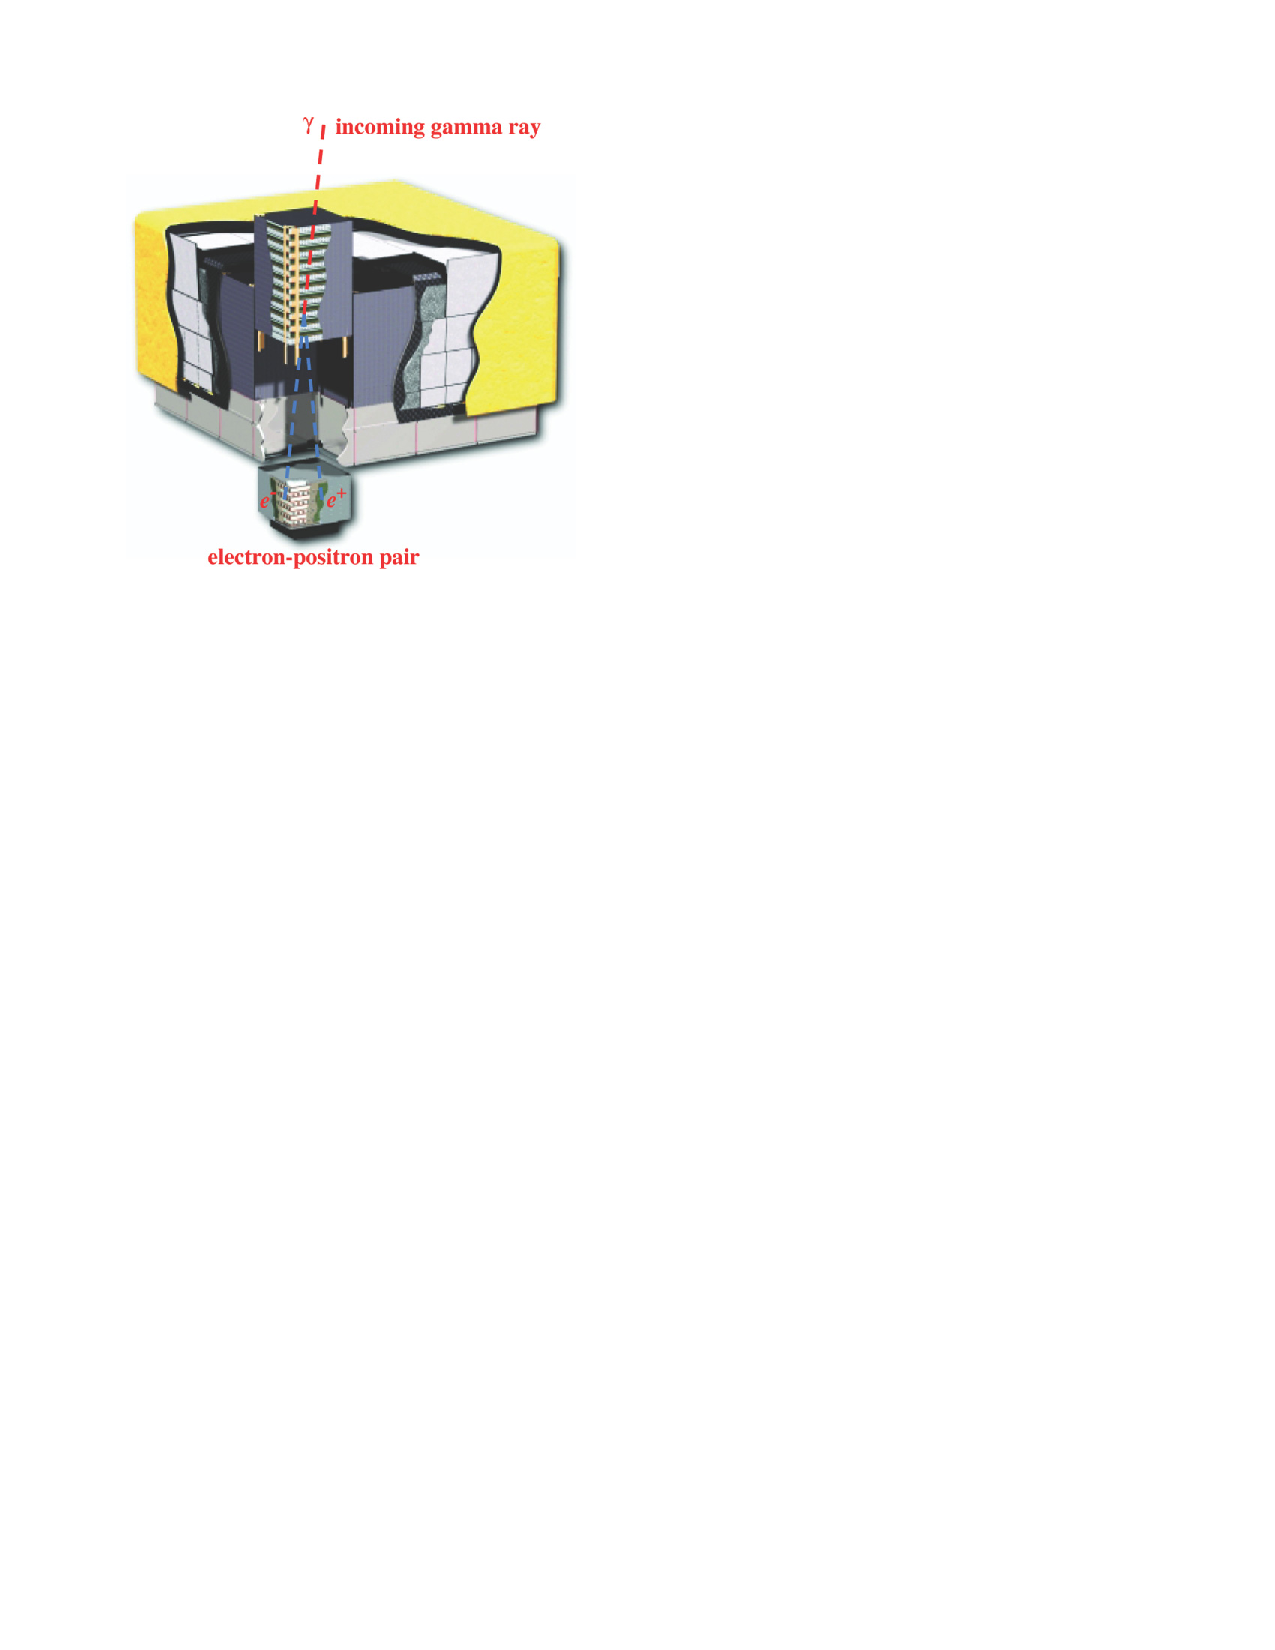
\includegraphics{chapters/introduction/figures/lat_detector_cutout.pdf}
  \caption{A schematic diagram of the \ac{LAT} with an incident $\gamma$-ray
    (red line) pair-converting into an electron and positron (blue lines)
    which are recorded in the tracker and calorimiter of the \ac{LAT}.
    This figure is taken from \citep{atwood_2009a_large-telescope}.  
  }
  \figlabel{lat_detector_cutout}
\end{figure} 


the \fermi Gamma-ray Space telescope was launched on June 11, 2008 on
a Delta II heavy launch vehicle \citep{atwood_2009a_large-telescope}.
The primary since instrument on board \fermi is the \ac{LAT},
which is a pair-conversion telescope which detects $\gamma$-rays in
the energy range from $20\unitspace\mev$ to $>300\unitspace\gev$.
\figref{lat_detector_cutout} shows a schematic diagram of the \ac{LAT}.

\todo[inline]{Put note about the \Acl{GBM} and how it is not that good.}

\subsection{The LAT Detector}

The tracker\ldots

The calorimiter\ldots

The \Ac{ACD} is \ldots


\subsection{Performance of the \acs{LAT}}

The \ac{LAT} has drastically improved our understanding of the high-energy
universe by offering an unprecidented view of the $\gamma$-ray sky.
It has an unprecidended effective area ($\sim9,500\unitspace\cm^2$),
single-photon energy resolution ($\sim10\%$), and single-photon
angular resolution ($\sim3\fdg5$ at $\energy=100\unitspace\mev$
and decreasing to $\lesssim0\fdg15$ for $\energy>10\unitspace\gev$)
\citep{atwood_2009a_large-telescope}.

With its $2.4\unitspace\steradian$ filed of view,

\todo[inline]{forward reference description of analysis of LAT data}
